\section{A fixed self-conjugate candidate}
\label{sec:candidate}

We now choose one diagram for the degree, before fixing a desired
constituent. The construction preserves self-conjugacy by attaching
transpose-matched cells to a staircase; its parameter bounds will
later make the two support tests exhaustive.

Set $N_0=0$ and choose the largest nonnegative $M$ for which
$N_M\le n$ and $N_M\equiv n\pmod2$,
and put
\begin{equation}\label{eq:parameters}
 r=\frac{n-N_M}{2},\qquad b=\left\lfloor\frac r2\right\rfloor,
 \qquad s=1+(r\bmod2),\qquad K=2M-1.
\end{equation}
Only $M\ge9$ will be used in this construction; smaller degrees will
be treated separately.

\begin{lemma}\label{lem:candidate}
The parameters satisfy
\begin{equation}\label{eq:r-bounds}
 r\le\begin{cases}(M-1)/2,&M\text{ odd},\\3M/2+2,&M\text{ even}.
 \end{cases}
\end{equation}
For $M\ge9$, the partition with column lengths
\begin{equation}\label{eq:candidate}
 L=(M+b+s-1,\ M-1+b,\ M-2,M-3,\ldots,3,\ 2^{b+1},\ 1^s)
\end{equation}
is self-conjugate and has size $n$. Consequently the support of
$S^L\otimes S^L$ is invariant under transposition of the target.
If no parity-compatible $M\ge9$ is available, then $n\le64$.
\end{lemma}

\begin{proof}
If $M$ is odd, the next triangular number of the same parity is
$N_{M+1}$, with difference $M+1$. Maximality gives
$2r\le M-1$. If $M$ is even, the next such number is $N_{M+3}$,
with difference $3M+6$, giving $2r\le3M+4$.

Relative to the staircase, the increments to the first two columns
sum to $2b+s-1$, and the added short columns have the same total.
Thus the size increases by $4b+2s-2=2r$. There are $M+b+s-1$
columns in total and $M+b-1$ columns of height at least two.
Counting those of height at least $j$ for $j\ge3$ gives successively
$M-2,M-3,\ldots,3$, followed by $b+1$ twos and $s$ ones.
These are exactly the column lengths in \eqref{eq:candidate}, so
$L=L^t$. It follows that
\[
 (S^L\otimes S^L)\otimes\sgn
 \cong S^L\otimes(S^L\otimes\sgn)
 \cong S^L\otimes S^L.
\]
Finally, every odd $n\ge45=N_9$ admits a parity-compatible index
at least nine, and every even $n\ge66=N_{11}$ admits one at least
eleven. The remaining degrees are at most $64$.
\end{proof}

Figure~\ref{fig:candidate} shows the matched additions in a small instance.
The path-incidence picture in Figure~\ref{fig:band-attachments} will
describe a different decomposition of the same construction.

\begin{figure}[ht]
\centering
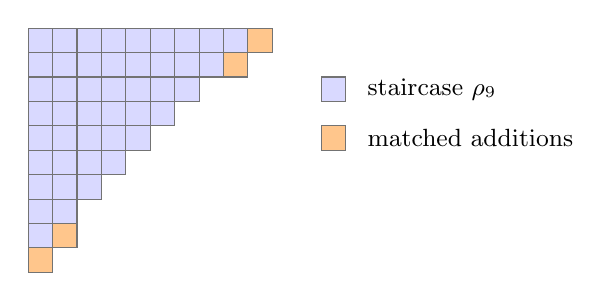
\begin{tikzpicture}[x=.31cm,y=-.31cm,every node/.style={font=\small}]
 \foreach \row/\width in {1/10,2/9,3/7,4/6,5/5,6/4,7/3,8/2,9/2,10/1}{
  \foreach \column in {1,...,\width}{
   \pgfmathtruncatemacro{\staircasecell}{\row+\column<=10}
   \ifnum\staircasecell=1
    \fill[blue!15] (\column-1,\row-1) rectangle (\column,\row);
   \else
    \fill[orange!45] (\column-1,\row-1) rectangle (\column,\row);
   \fi
   \draw[black!55] (\column-1,\row-1) rectangle (\column,\row);
  }
 }
 \fill[blue!15] (12,2) rectangle (13,3);
 \draw[black!55] (12,2) rectangle (13,3);
 \node[right] at (13.5,2.5) {staircase $\rho_9$};
 \fill[orange!45] (12,4) rectangle (13,5);
 \draw[black!55] (12,4) rectangle (13,5);
 \node[right] at (13.5,4.5) {matched additions};
\end{tikzpicture}
\caption{The degree-$49$ candidate with $M=9$, $r=2$, $b=1$, and
$s=1$. Its row and column lengths are both
$(10,9,7,6,5,4,3,2,2,1)$. The four added cells come in transposed
pairs, preserving self-conjugacy.}
\label{fig:candidate}
\end{figure}

When $r=0$, the candidate is the staircase itself, and
Theorem~\ref{thm:cyclic-input} already supplies all constituents.
For $r>0$ we give two sufficient support tests. For a target $\nu$,
write its column heights and row lengths as
\[
 h=(h_1,h_2,\ldots)=\nu^t,\qquad
 w=(w_1,w_2,\ldots)=\nu,
\]
with zeros appended. Both tests refer to the single square
$S^L\otimes S^L$ fixed above. We are free to interchange $h$ and $w$
by Lemma~\ref{lem:candidate}.

The coverage has four steps. A small first-four row or column sum is
handled by Proposition~\ref{prop:balance-four}. Otherwise the band
criterion covers every $M\ge22$ and all intermediate parameters apart
from the nineteen pairs in \eqref{eq:capacity-exceptions}; the exact
capacity check handles those pairs. Proposition~\ref{prop:finite-check}
handles all eligible degrees at most $64$, completing the small-index
remainder. The two finite checks thus have separate, explicitly bounded
roles.
